\subsection{The Server Application}
As previously mentioned, the backend will be utilizing Amazon Web Services. To keep the design as
simple as possible, all required services will be using AWS, especially since all of the services
integrated very nicely with one another. In order to allow our LoRaWAN devices to communicate to the
backend, they will need to connect to a LoRaWAN Network Server, and have that talk to the rest of
our services. AWS provides multiple services relating to IoT, specifically LoRaWAN.

\subsubsection{The Backend Application Software Stack}
The front facing user web application will be the main way of interfacing and managing the nodes, as
well as viewing the measured data in a visual and graphical format. The application will need to
allow the user to login, and manage their own nodes. They should also be able to remotely control
them, view analytics, such as the time last seen, its approximate location, and the individual
packets. The user should also be able to configure notification settings. The notification types
will be email, SMS, and Twitter, which will all be provided by Amazon's Simple Notification Service
(SNS), as shown in Figure \ref{server-stack}. 

The website will be hosted through the AWS Amplify
service, and the API endpoints to interface with the backend to retrieve sensor data, device
configuration, and other important pieces of information and configuration will be implemented
through the AWS API Gateway service. These two services make up the "Web Server and Backend
Interface" layer in the figure. The "Application Supporting Services" layer is composed of services
that help bridge the gap between the IoT layers and the web app layers. The Amazon DynamoDB is
a NoSQL database, and is where the API gateway, AWS Lambda, and AWS IoT Events will share data. The
Amazon Cognito user authentication is for logging in users in securely. 

AWS IoT Events provides a rule making service for identifying and notifying of extenuating
circumstances from data received from IoT devices on the network. This service will be utilized to
help create the email, SMS, and/or Twitter alerts as previously mentioned. Events and rules, just
like the rule engine in the IoT Core service, use an SQL-like language to specify how to read data
and how to act on it. The difference between IoT Events and the IoT rule engine is that IoT Events
can be used for identifying issues for groups of IoT devices, and is continuously monitoring devices
for failures, or other special case. The IoT rule engine, however, is for routing incoming MQTT
messages to AWS Lambda, or other services to be further processed. IoT Events can also integrate
with AWS Lambda and other services, but its use cases are entirely different. AWS Lambda is
a server-less computing engine service. In computing, lambdas are functions that can be passed
around like variables, and can be created at runtime.

AWS Lambda allows the developer to write functions that can be instantiated, and automatically
previsioned in the cloud, whenever an event or other service requests one. For example, AWS Lambdas
could be used to decode binary MQTT messages into JSON, or another human-readable format. The web
server, AWS Amplify, could also request Lambdas to be execute, not just the IoT core. The last layer
in the backend stack is the "LoRaWAN Network Server, MQTT Broker, IoT Services" layer. Here, the
LoRaWAN Network Server is run, along with services to accept and send MQTT messages, manage devices,
and route MQTT messages to other services. This is the layer that the LoRaWAN gateway packet
forwarder will directly talk to.

As for the web front-end, the React JavaScript framework will be utilized with Typescript to quickly
and more easily catch errors before deployment. React is a component-based JavaScript framework
originally developed by Facebook. It provides a virtual DOM (document object model), so that only
specific parts of a web page are updated when the data behind them do. This is unlike how some
traditional JavaScript-only, DOM-driven websites were developed previously. Without a virtual DOM,
it's impossible to safely know how changing data might affect the whole page, so the whole DOM was
updated every time the state changed. React has a plentiful ecosystem of plugins, additional
libraries, and tons of additional documentation and help online from the huge community it has
garnered.

\begin{figure}
  \centering
  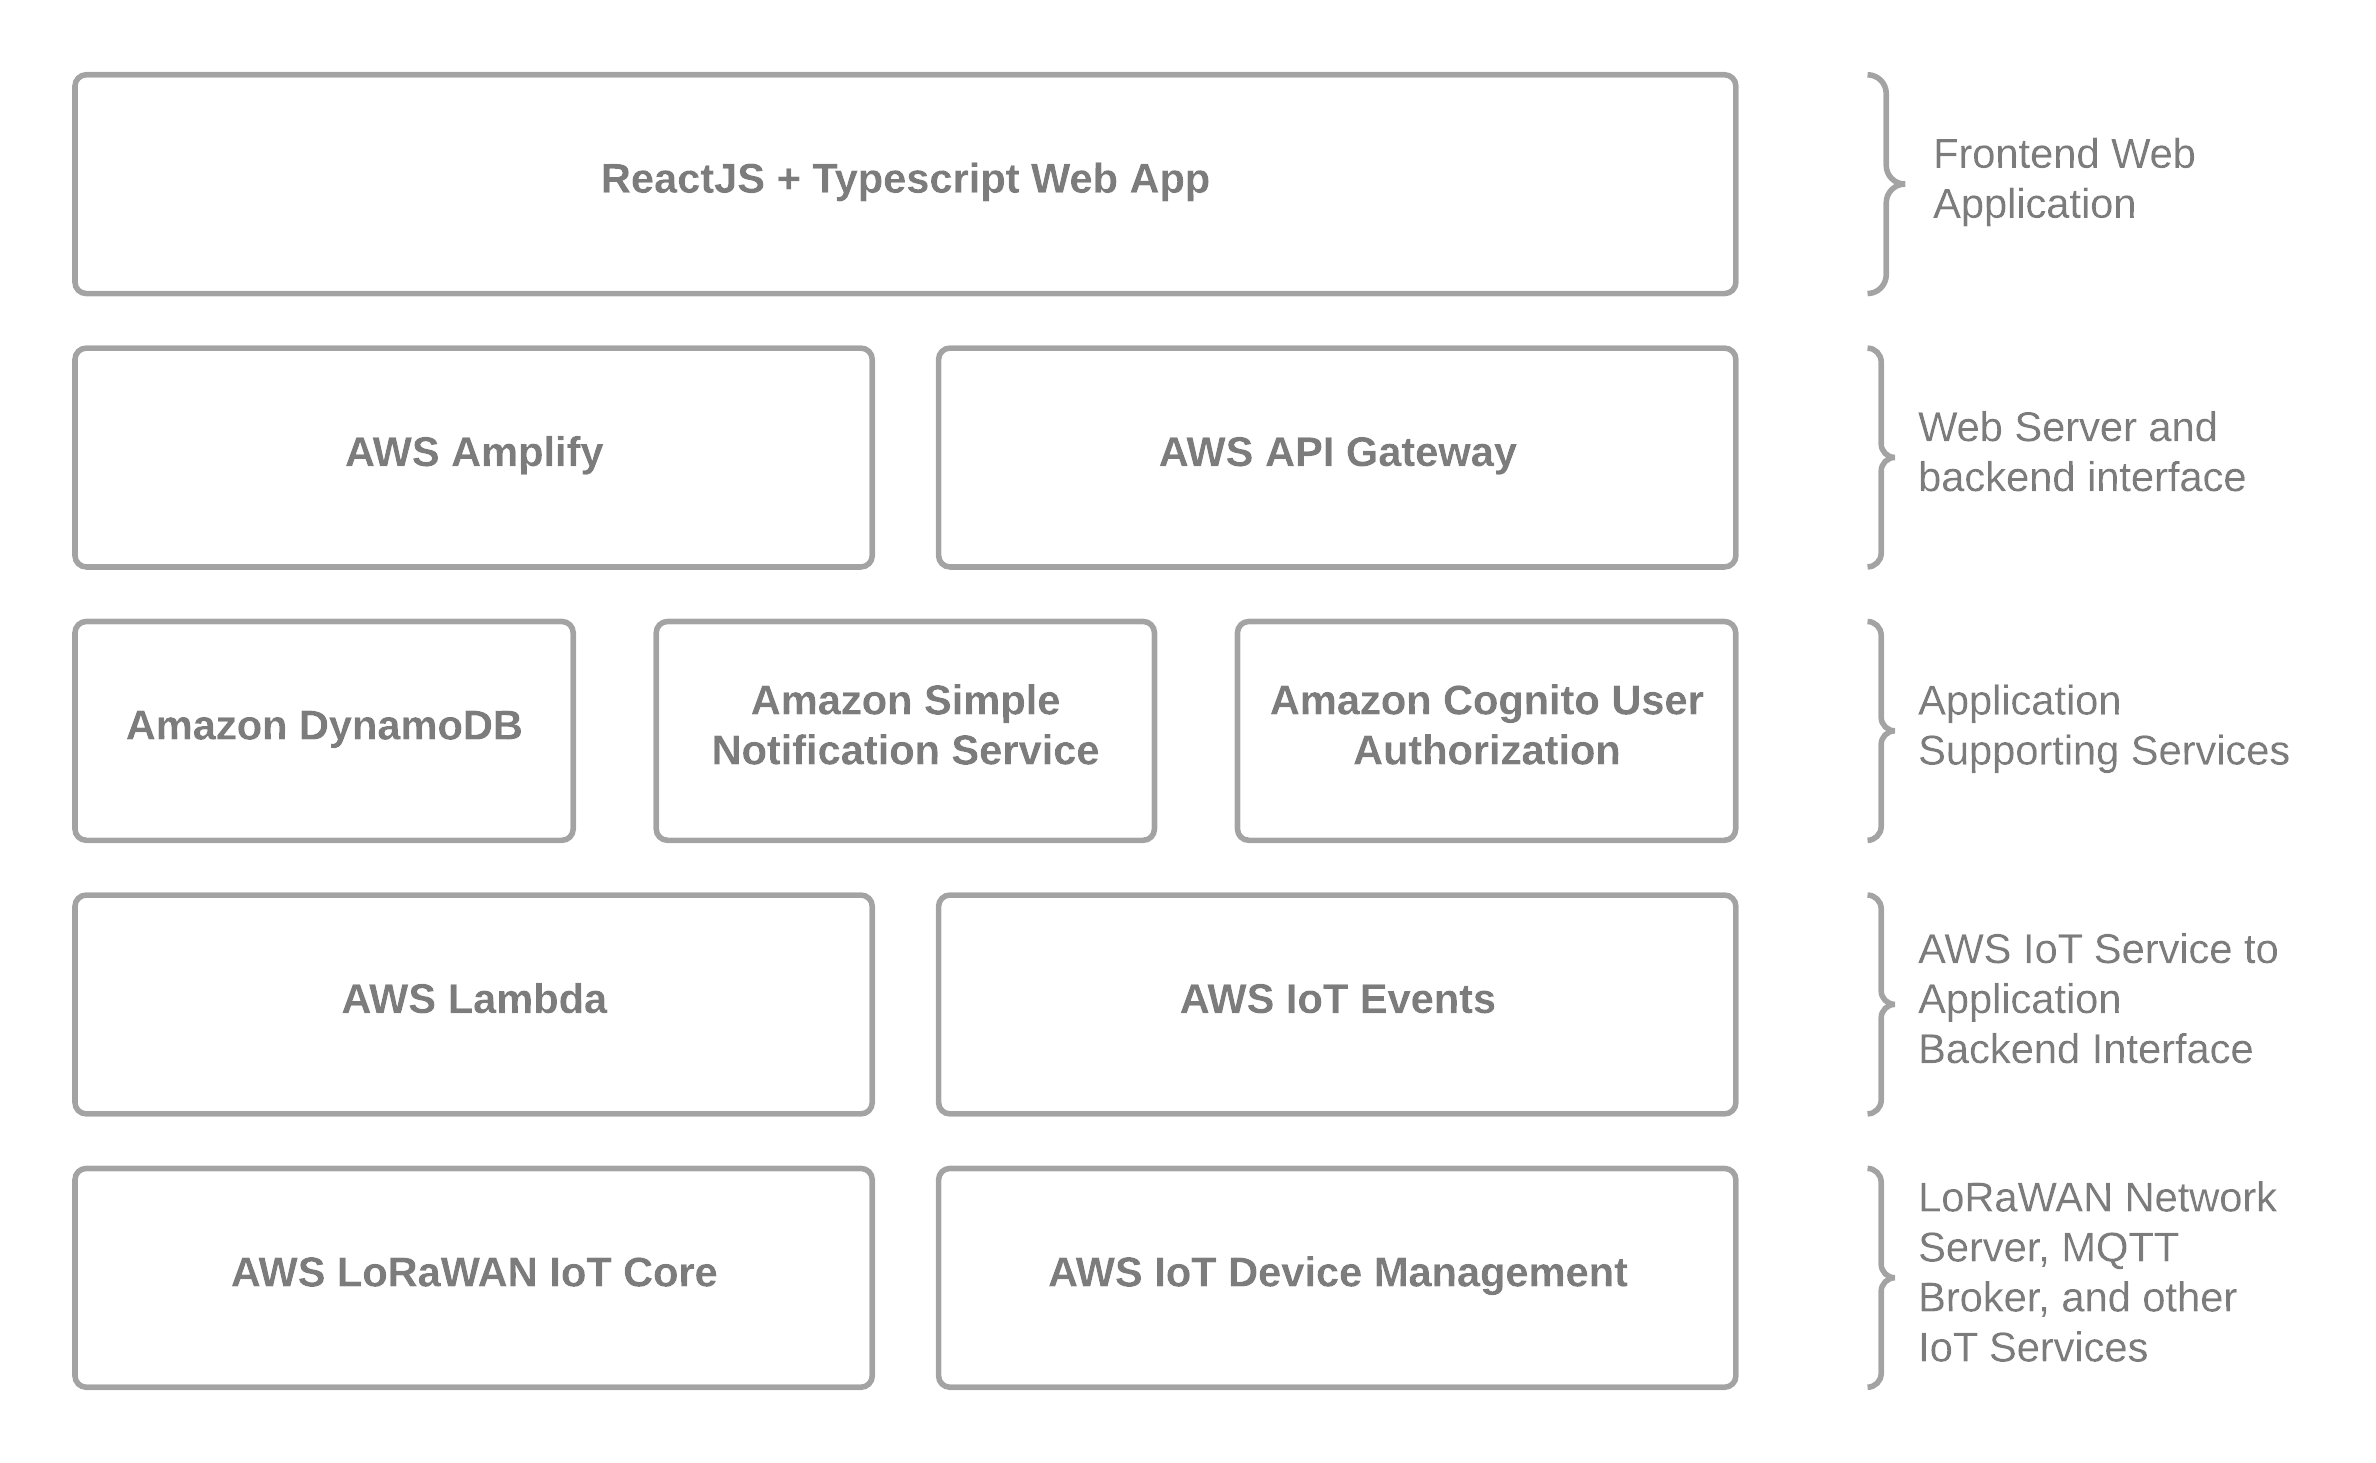
\includegraphics[width=5in]{server-stack}
  \caption{Backend Server and Web Application Stack}
  \label{server-stack}
\end{figure}


\subsubsection{The REST API}
The backend will need to expose many API endpoints for the webapp to display sensor and device data.
The frontend will be able to retrieve data regarding the location of the sensor nodes, the data and
logs from each node, and send commands to the nodes. The API should also allow users to login,
register their devices to the AWS LNS, Helium and/or The Things Network.

